\documentclass[a4paper, 11pt]{article}
\usepackage[utf8]{inputenc}
\usepackage[english]{babel}
\usepackage[utf8]{inputenc}
\usepackage[margin=2.cm]{geometry}
\usepackage{fancyhdr}

\usepackage[T1]{fontenc}
\usepackage{lmodern}

\usepackage{graphicx}
\graphicspath{ {images/} }
\usepackage{pdflscape}


\usepackage{array}

\usepackage{multirow}

\usepackage{color,array}

\definecolor{mygray}{gray}{0.6} %custom color for text

\usepackage{float}
\usepackage[table,xcdraw]{xcolor}


\usepackage{varwidth} %for lists next to each other

%for subfigure
\usepackage{subcaption}


%Includes "References" in the table of contents
\usepackage[nottoc]{tocbibind}

\usepackage{enumitem}
\setlist{nolistsep}

\fancypagestyle{plain}{%
  \renewcommand{\headrulewidth}{0pt}%
  \fancyhf{}%
  \fancyfoot[L]{\footnotesize Raymond Lochner}
  \fancyfoot[C]{\footnotesize December 2017 - Université libre de Bruxelles}%
  \fancyfoot[R]{\thepage}
}
\pagestyle{plain}

\date{\today}

\begin{document}

\begin{titlepage}
	\centering
	{\scshape\LARGE Université libre de Bruxelles \par}
	\vspace{1cm}
	{\scshape\Large INFO-F-409 - Learning Dynamics\par}
	\vspace{1.5cm}
	{\huge\bfseries {Assignment Three\par}}
	\vspace{0.5cm}
	{\Large Multi-Armed Bandits\par}
	\vspace{2cm}
	{\Large Raymond Lochner - 000443637\par}
	\vspace{0.5cm}
	{\Large raymond.lochner@ulb.ac.be}
	\vfill
	
	\setcounter{tocdepth}{2} %hides subsubsections in TOC
	\tableofcontents

\vfill
% Bottom of the page
	{\large \today \par}
\end{titlepage}

\newpage

\section*{Preliminary information}

Every experiment was run 2000 times and the results averaged

\section{Exercise 1}
\subsection{Combined Average Reward}

\begin{figure}[H]
	\centering
    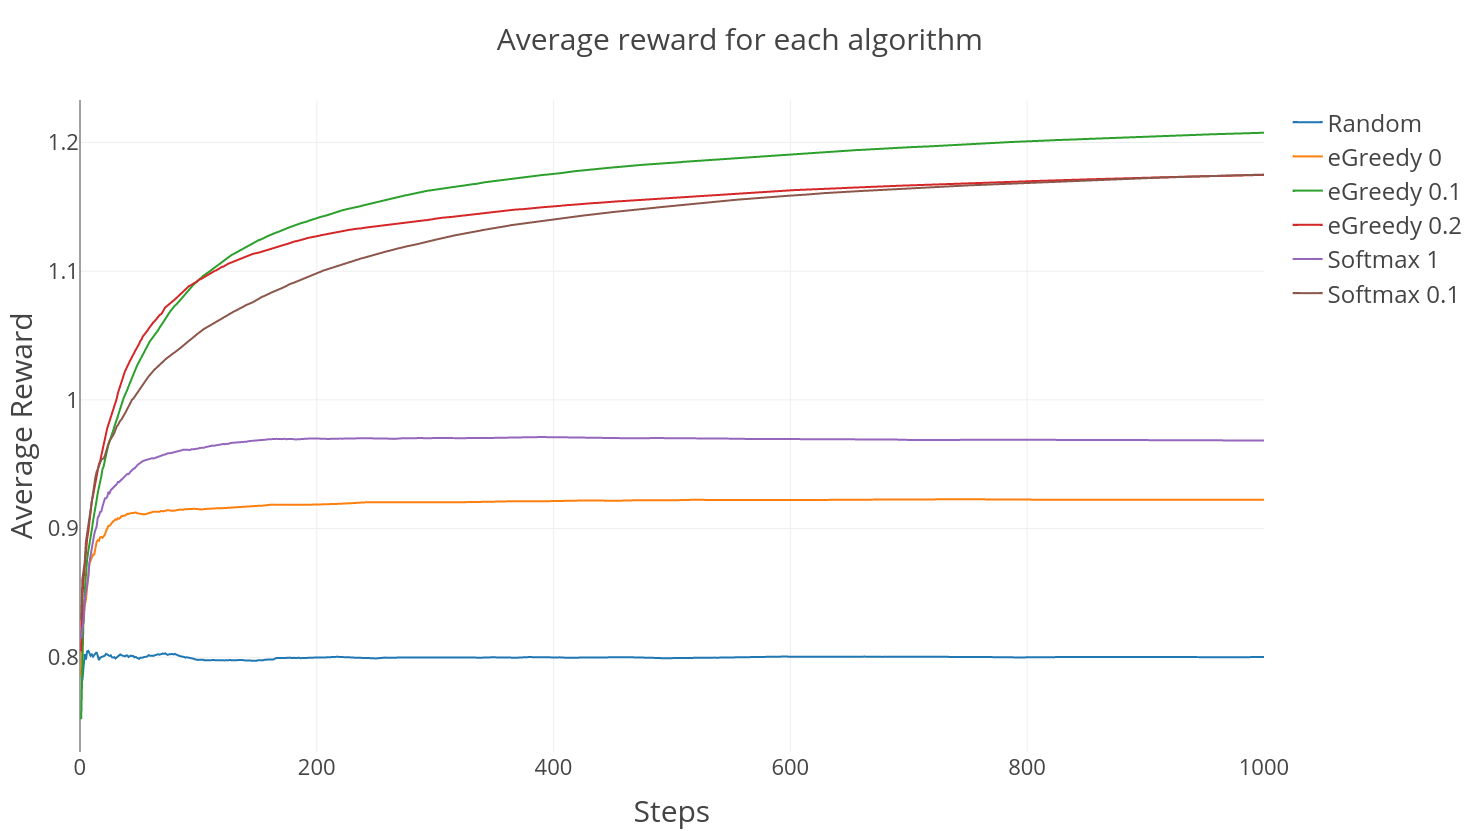
\includegraphics[width=1\linewidth]{ex1_1_average_rewards}
    %\caption{Two Neighborhood types}
\end{figure}

\subsection{Q* values for each arm}

\begin{figure}[H]
	\centering
    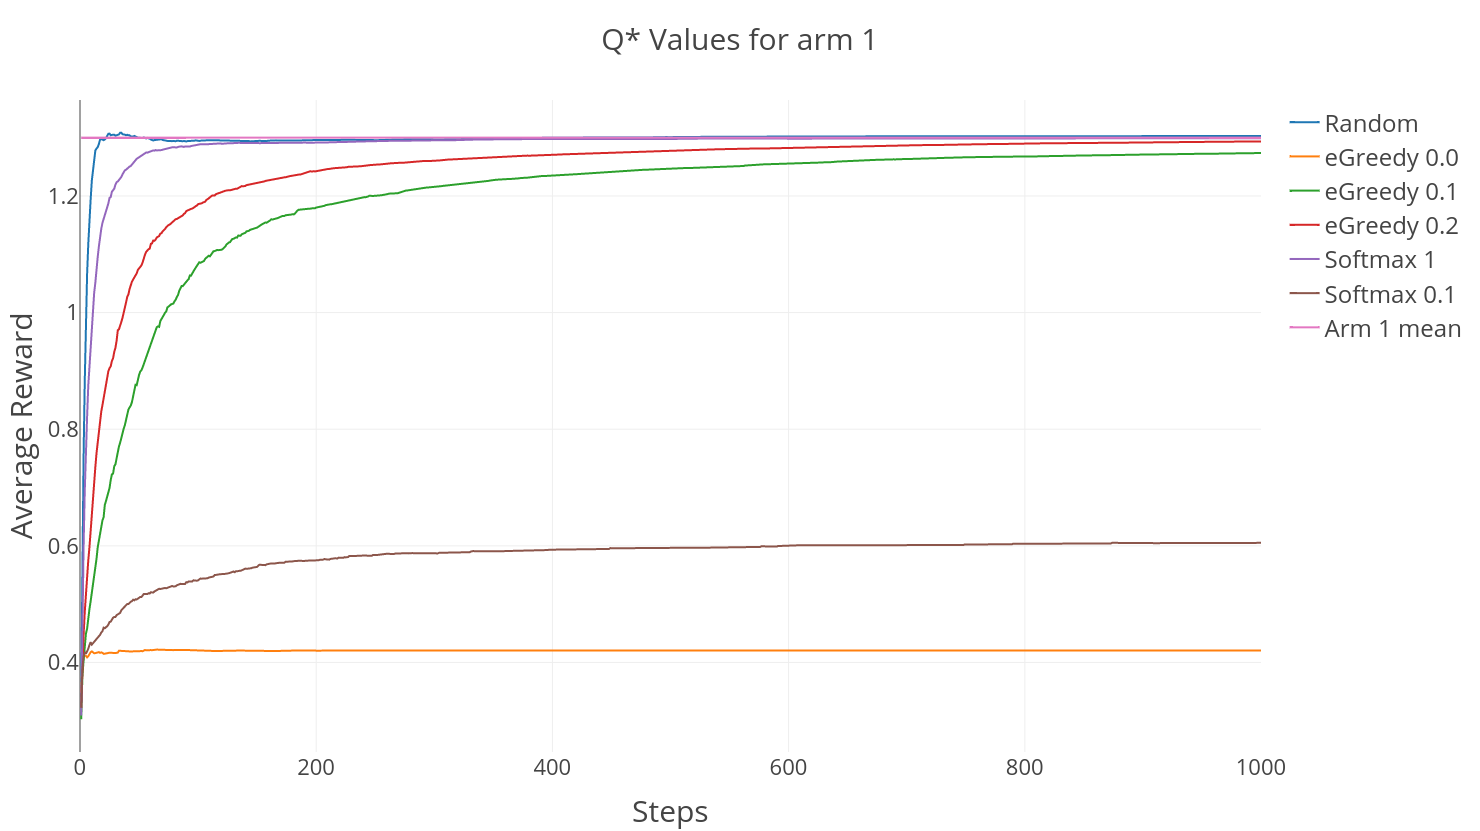
\includegraphics[width=1\linewidth]{ex1_Q1_reward}
    %\caption{Two Neighborhood types}
\end{figure}

\begin{figure}[H]
	\centering
    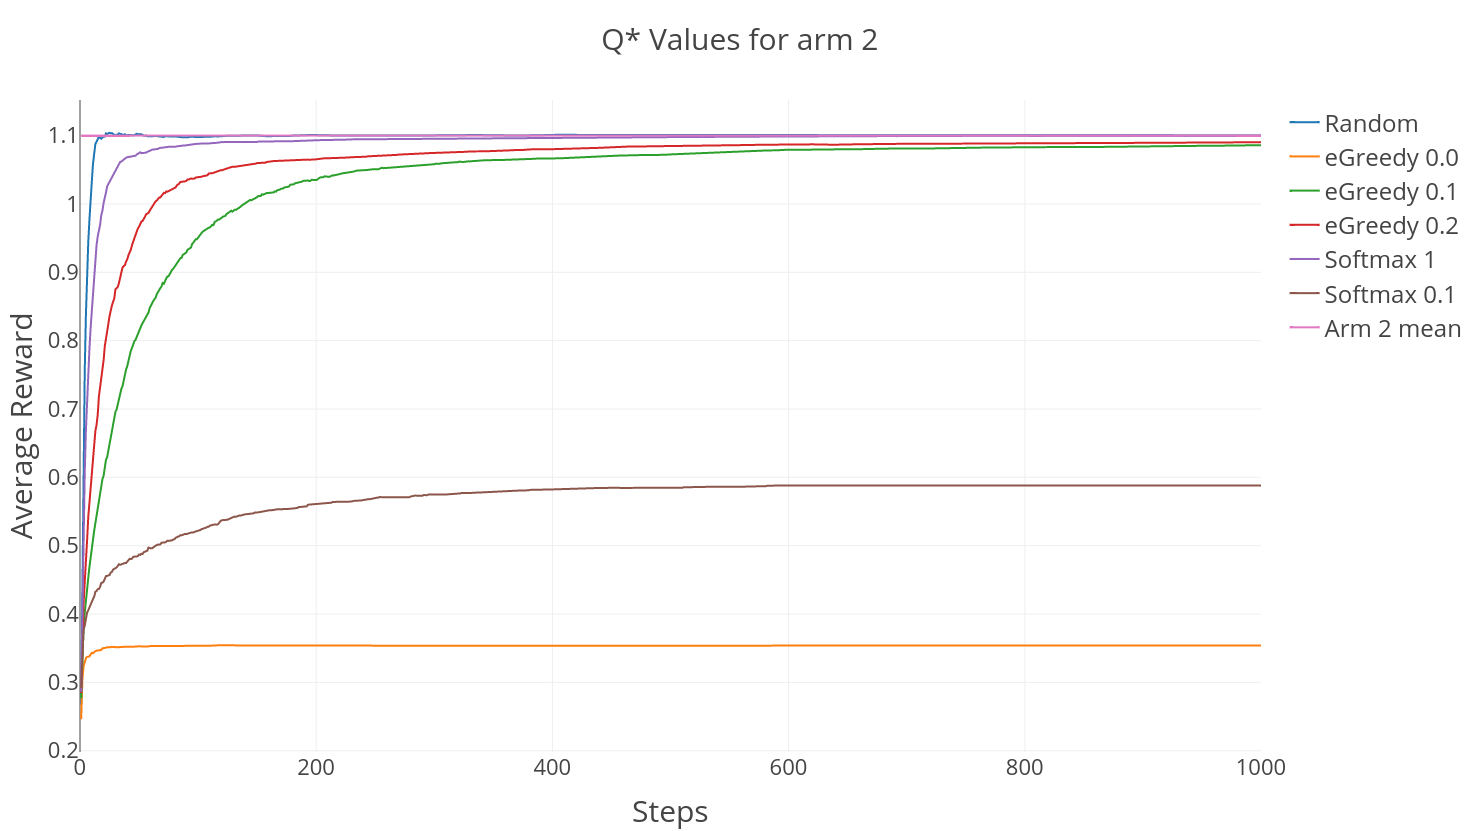
\includegraphics[width=1\linewidth]{ex1_Q2_reward}
    %\caption{Two Neighborhood types}
\end{figure}

\begin{figure}[H]
	\centering
    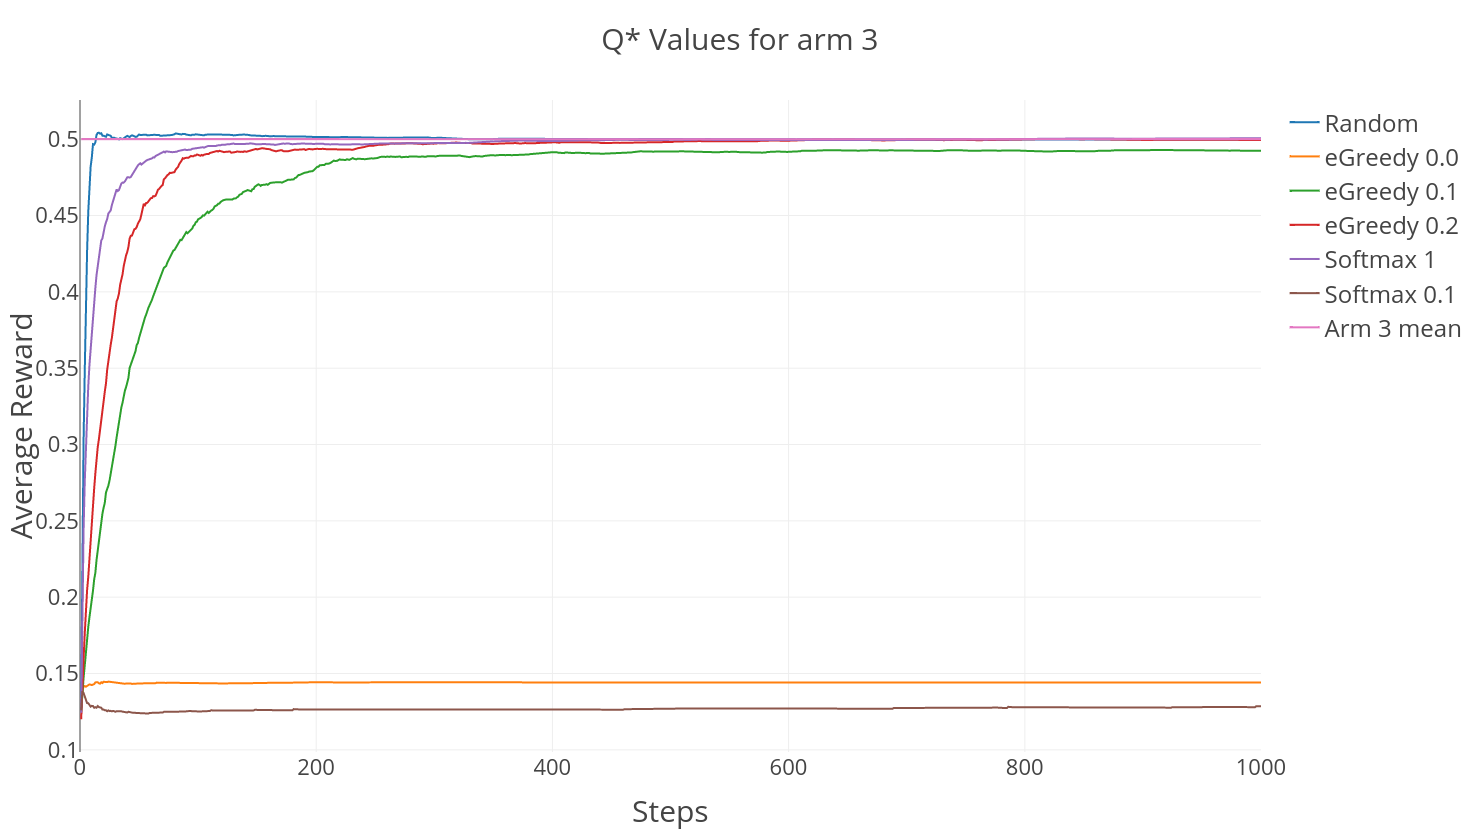
\includegraphics[width=1\linewidth]{ex1_Q3_reward}
    %\caption{Two Neighborhood types}
\end{figure}

\begin{figure}[H]
	\centering
    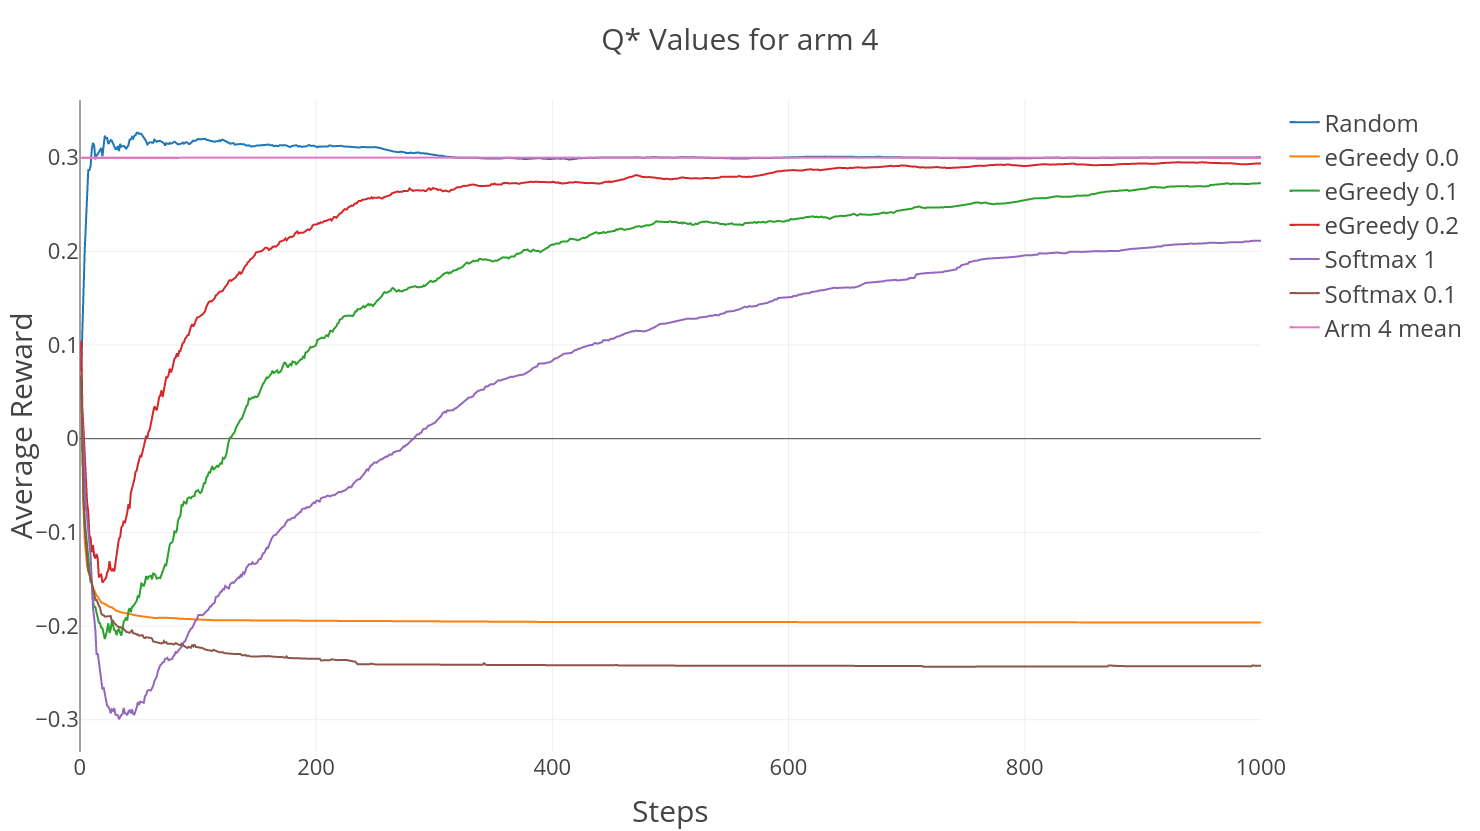
\includegraphics[width=1\linewidth]{ex1_Q4_reward}
    %\caption{Two Neighborhood types}
\end{figure}

\subsection{Histogram on actions chosen}

\begin{figure}[H]
\centering
\begin{subfigure}{.5\textwidth}
  \centering
  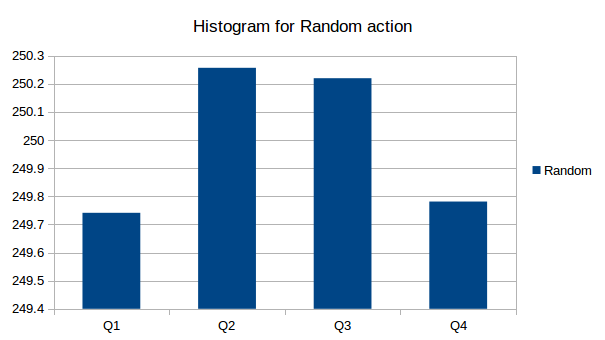
\includegraphics[width=1\linewidth]{ex1_histogram_random}
\end{subfigure}%
\begin{subfigure}{.5\textwidth}
  \centering
  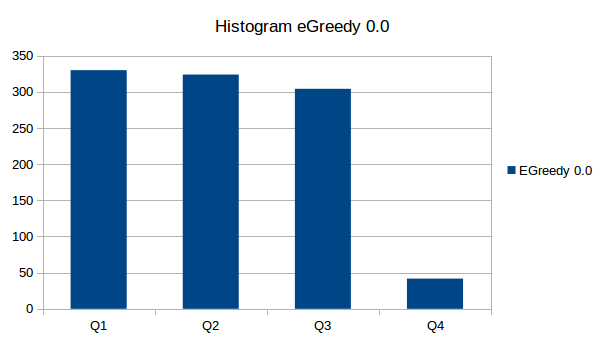
\includegraphics[width=1\linewidth]{ex1_histogram_egreedy00}
\end{subfigure}%

\begin{subfigure}{.5\textwidth}
  \centering
  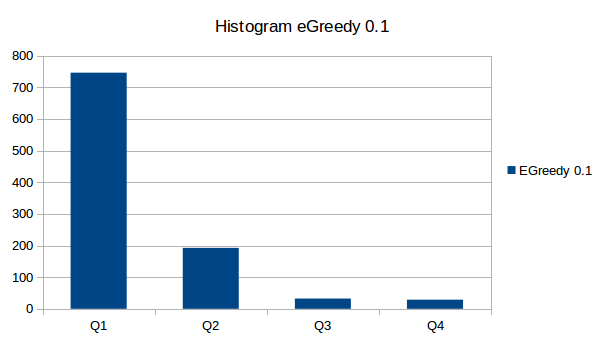
\includegraphics[width=1\linewidth]{ex1_histogram_egreedy01}
\end{subfigure}%
\begin{subfigure}{.5\textwidth}
  \centering
  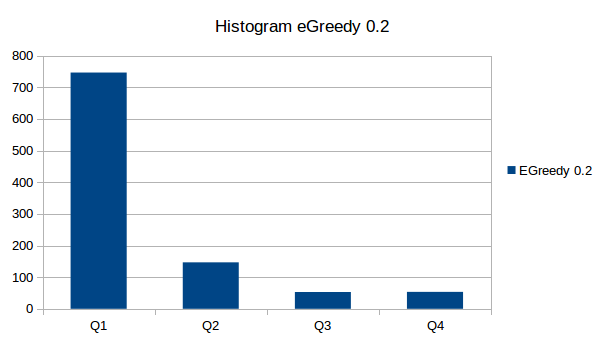
\includegraphics[width=1\linewidth]{ex1_histogram_egreedy02}
\end{subfigure}%

\begin{subfigure}{.5\textwidth}
  \centering
  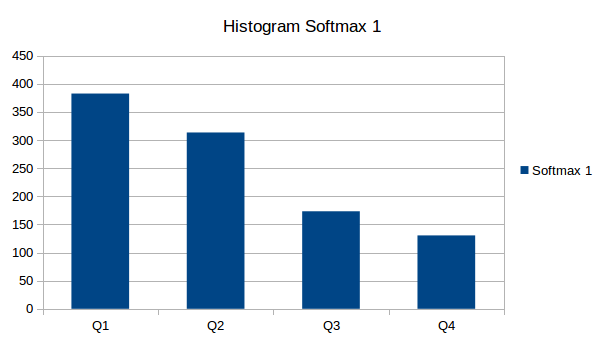
\includegraphics[width=1\linewidth]{ex1_histogram_softmax1}
\end{subfigure}%
\begin{subfigure}{.5\textwidth}
  \centering
  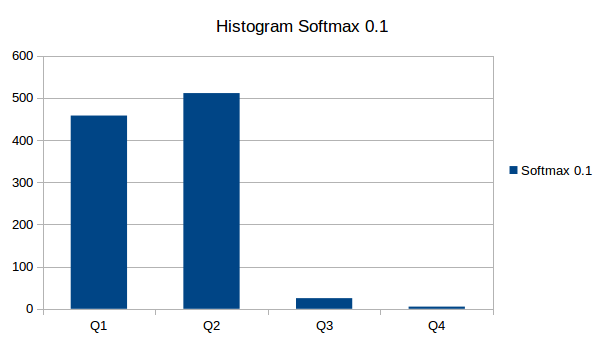
\includegraphics[width=1\linewidth]{ex1_histogram_softmax01}
\end{subfigure}%
\end{figure}


\subsection{Results}

We observe the combined average reward figure: The \textit{eGreedy 0.1} method has the highest average reward after 100 steps until the end of the simulation of 1000 steps. \textit{eGreedy 0.2} and \textit{Softmax 0.1} share the second place together. \textit{Softmax 1} comes in fourth place, \textit{eGreedy 0.0} on fifth and the random algorithm last.

These results can also be observed by looking at the histograms where \textit{eGreedy 0.1} has the highest arm 1 selection.

The random algorithm arrives the fastest at determining the Q* value for every arm but does not yield a good  average. This could indicate that random exploration is a good method in the beginning but has to stop after some steps to select a single arm afterwards to earn the maximum award.

The graphs that show the Q* values for each arm show us that the two methods \textit{eGreedy 0.0} and \textit{Softmax 0.1} are not exploring enough in the beginning as they do not arrive at the actual Q* value and are stuck with a action they selected in the very beginning. This is due to the fact that we are initializing all Q* values to 0 at step 0 which results in the algorithm sticking to one action with a very high percentage without having explored the other actions.

%%%%%%%%%%%%%%%%%%%%%%%%%%%%%%%%%%%%%%%%%%%%%%%%%%%%%%%%%%%%%%%%%%%%%%%%%%%%%%%%
%%%%%%%%%%%%%%%%%%%%%%%%%%%%%%%%%%%%%%%%%%%%%%%%%%%%%%%%%%%%%%%%%%%%%%%%%%%%%%%%
\section{Exercise 2}

\subsection{Combined Average Reward}

\begin{figure}[H]
	\centering
    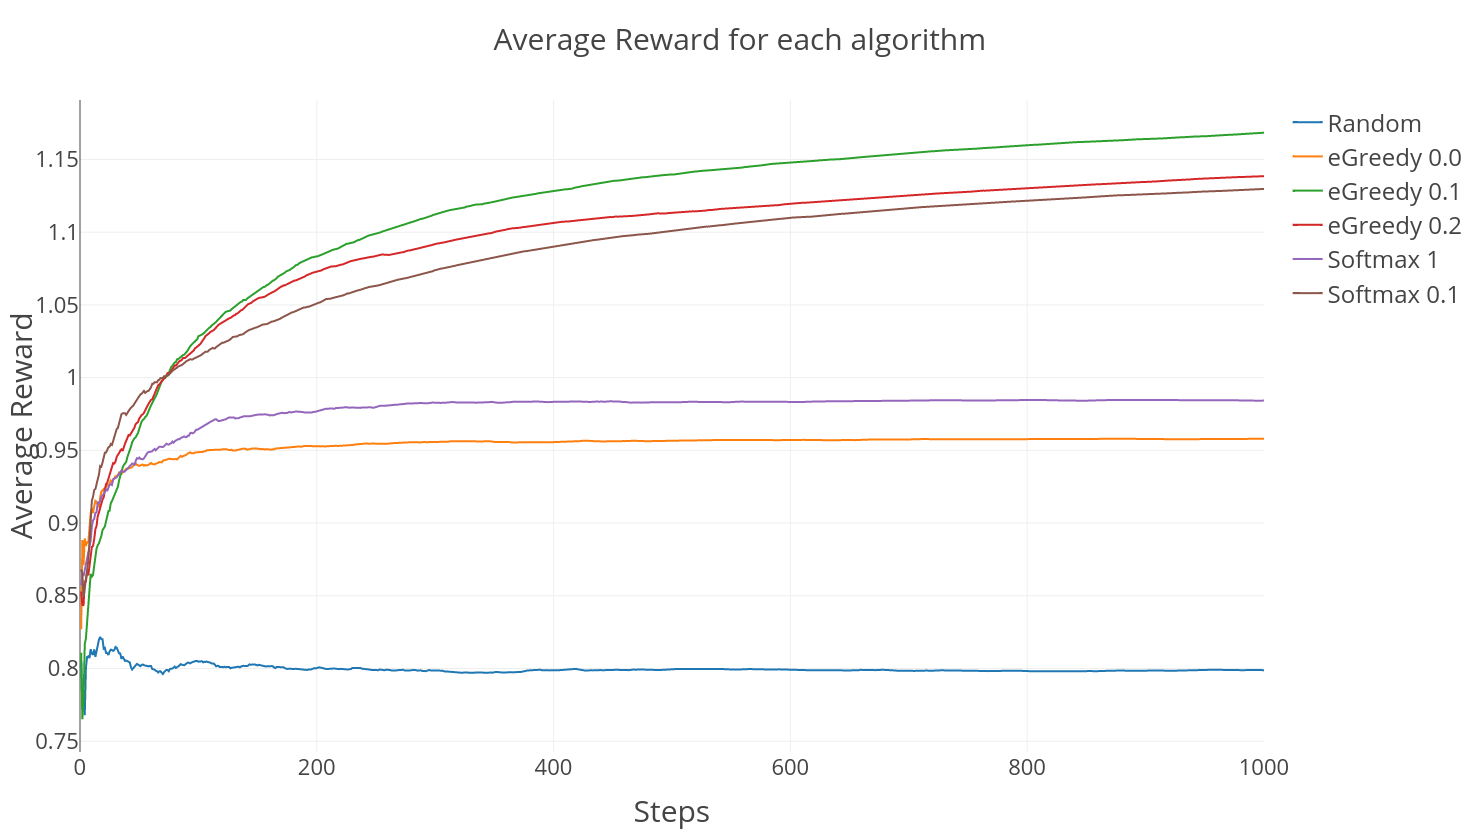
\includegraphics[width=1\linewidth]{ex1_2_average_rewards}
    %\caption{Two Neighborhood types}
\end{figure}

\subsection{Q* values for each arm}

\begin{figure}[H]
	\centering
    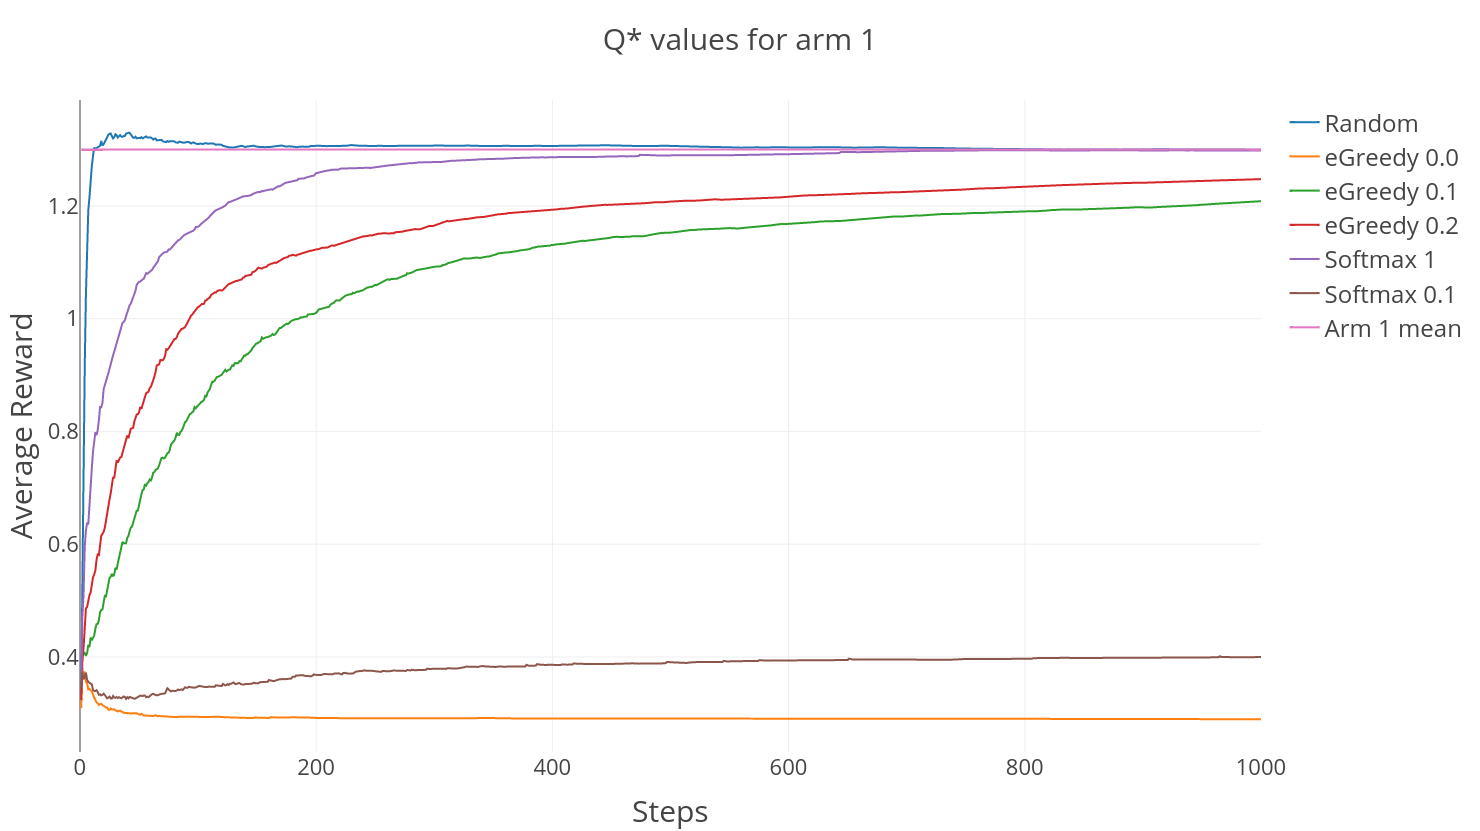
\includegraphics[width=1\linewidth]{ex1_2_Q1_reward}
    %\caption{Two Neighborhood types}
\end{figure}

\begin{figure}[H]
	\centering
    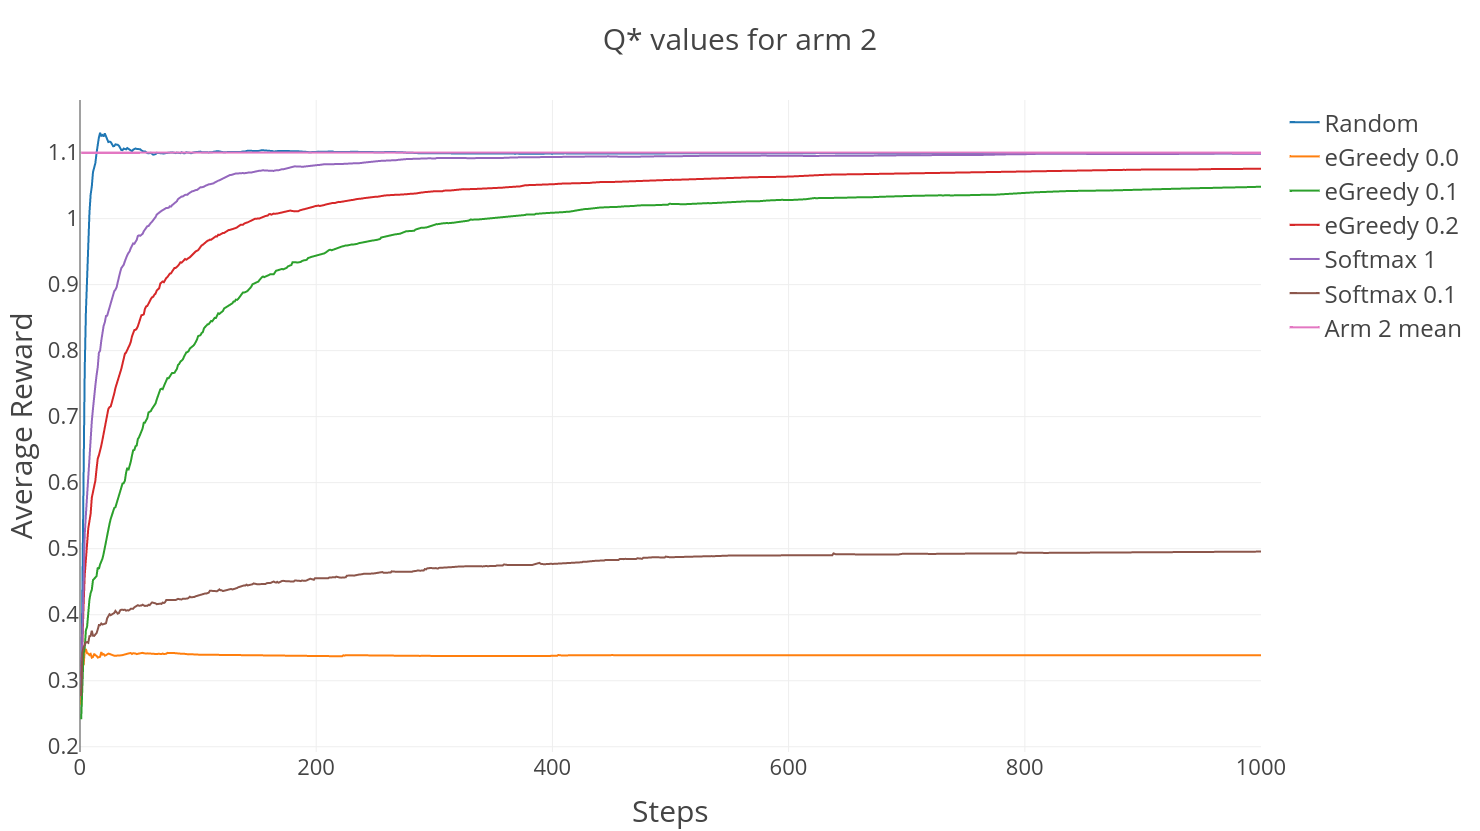
\includegraphics[width=1\linewidth]{ex1_2_Q2_reward}
    %\caption{Two Neighborhood types}
\end{figure}

\begin{figure}[H]
	\centering
    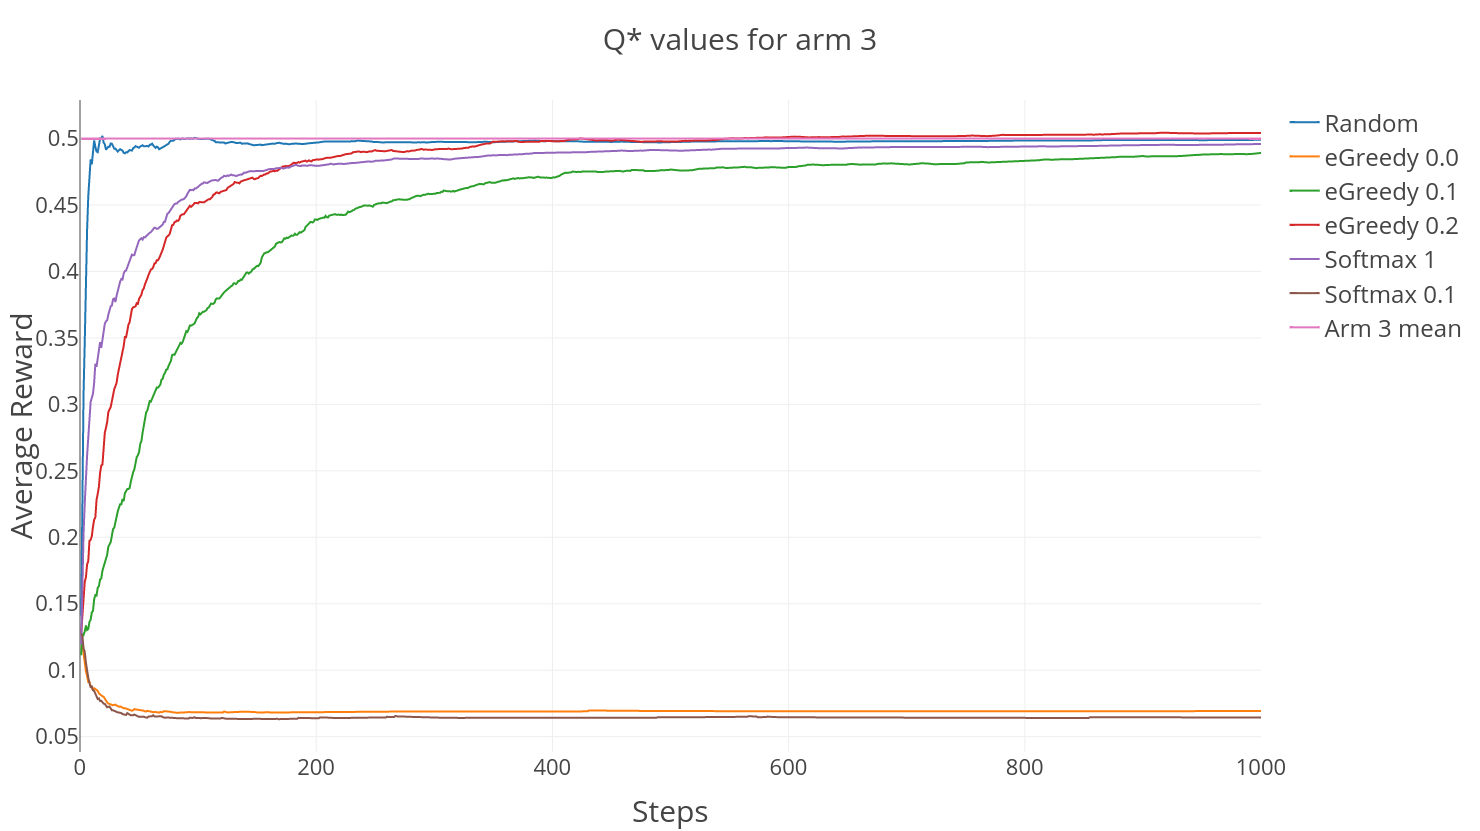
\includegraphics[width=1\linewidth]{ex1_2_Q3_reward}
    %\caption{Two Neighborhood types}
\end{figure}

\begin{figure}[H]
	\centering
    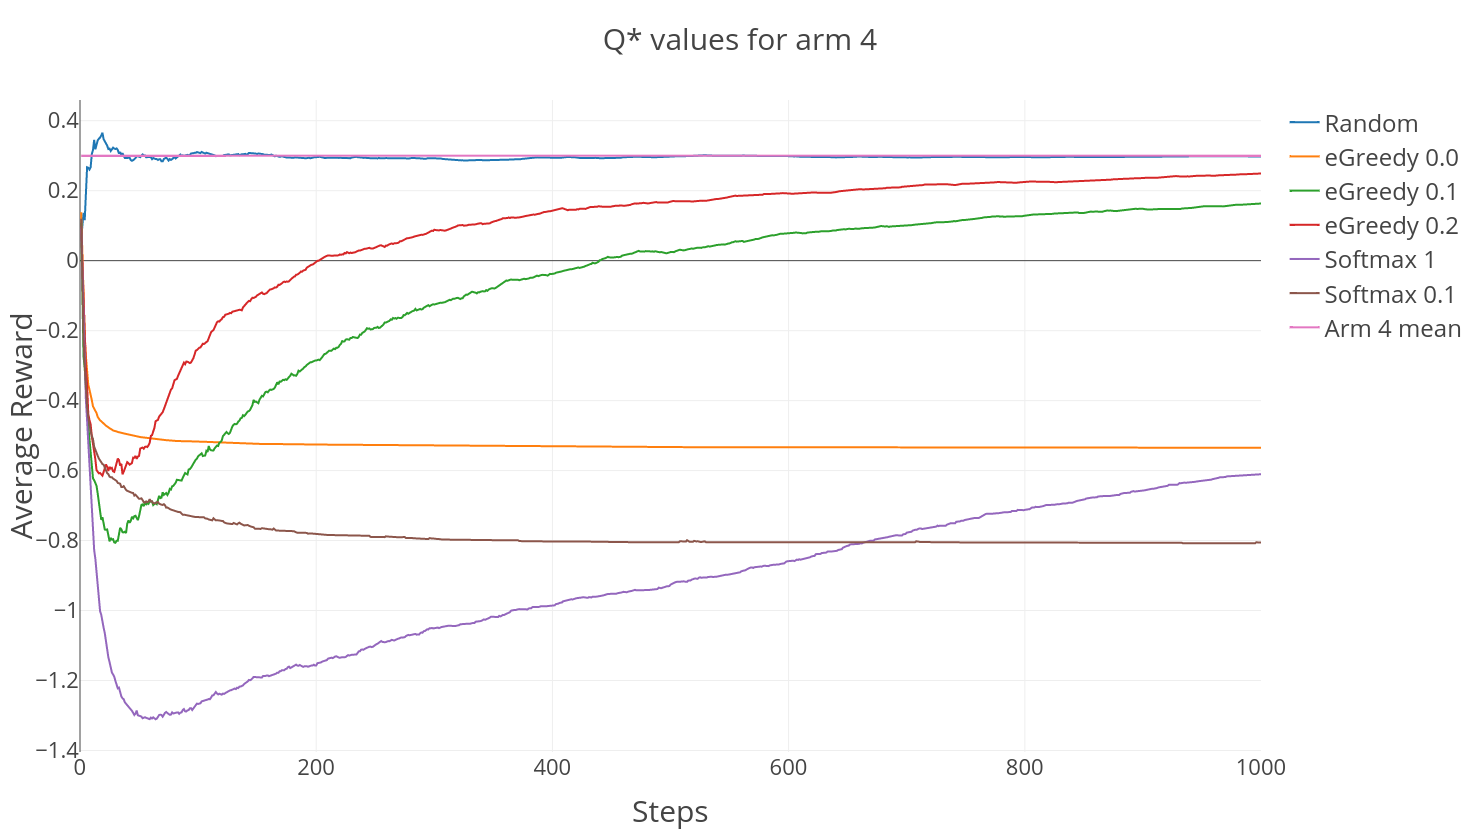
\includegraphics[width=1\linewidth]{ex1_2_Q4_reward}
    %\caption{Two Neighborhood types}
\end{figure}

\subsection{Histogram on actions chosen}

\begin{figure}[H]
\centering
\begin{subfigure}{.5\textwidth}
  \centering
  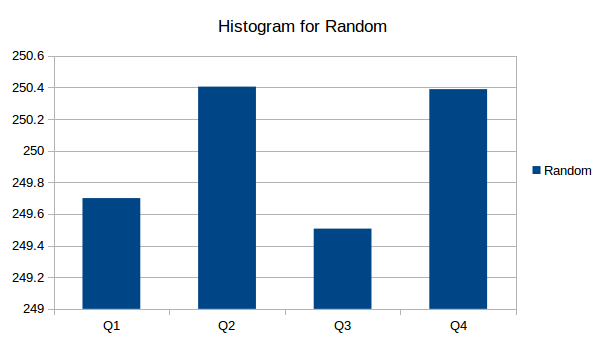
\includegraphics[width=1\linewidth]{ex1_2_histogram_random}
\end{subfigure}%
\begin{subfigure}{.5\textwidth}
  \centering
  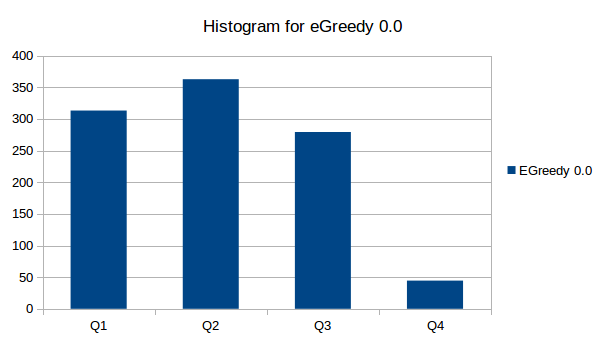
\includegraphics[width=1\linewidth]{ex1_2_histogram_egreedy00}
\end{subfigure}%

\begin{subfigure}{.5\textwidth}
  \centering
  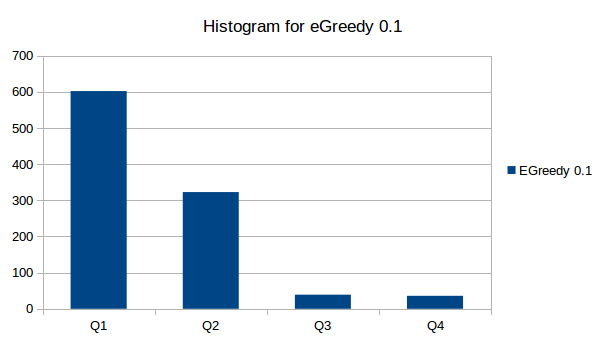
\includegraphics[width=1\linewidth]{ex1_2_histogram_egreedy01}
\end{subfigure}%
\begin{subfigure}{.5\textwidth}
  \centering
  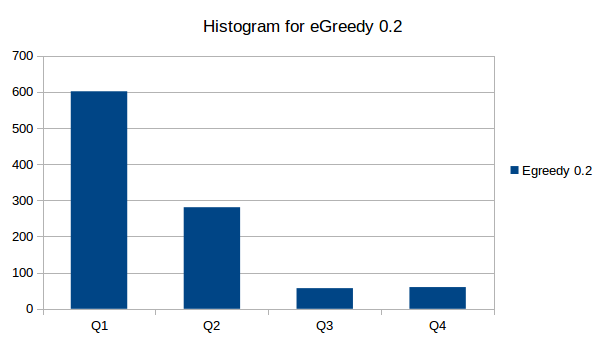
\includegraphics[width=1\linewidth]{ex1_2_histogram_egreedy02}
\end{subfigure}%

\begin{subfigure}{.5\textwidth}
  \centering
  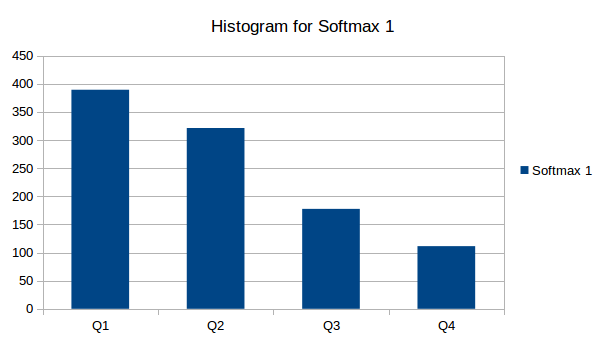
\includegraphics[width=1\linewidth]{ex1_2_histogram_softmax1}
\end{subfigure}%
\begin{subfigure}{.5\textwidth}
  \centering
  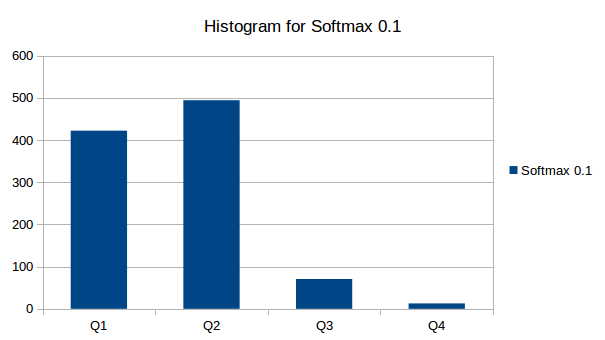
\includegraphics[width=1\linewidth]{ex1_2_histogram_softmax01}
\end{subfigure}%
\end{figure}

\subsection{Results}


Doubling the deviation does not change the order of best algorithms with 1000 steps. The problem is harder to learn as the Q* values are similar to exercise one, but they are doing so with more steps.

The performance, or total reward after 1000 steps influences the used algorithms differently. It decreases the reward for the \textit{eGreedy 0.1} and \textit{eGreedy 0.2} methods but increases the reward slightly for the \textit{Softmax 0.1} method.


The average reward per algorithm is lower than compared to the first exercise. This can be explained due to the fact that the doubling of the deviation makes the Q* values more \textit{random} and hence influences the probability of lower performing arms to be chosen in the beginning.







\end{document}